\subsection{Adding Settings to \giraf}\label{sec:sprint3:designsettings}
The idea behind providing a way to change settings from \launcher for both itself, but also other \giraf applications, is to create a streamlined and uniform user interface for changing settings across the entire project.
This section discusses how to design the architecture of what will be an activity in Android, implemented in the context of \launcher, to contain the settings.

\subsubsection{Choosing Between Prototypes}
As discussed in \cref{sec:sprint2:secondmeeting}, the clients agreed that settings should be accessible through two methods:

\begin{itemize}
	\item A dialogue box in each individual application, containing only settings relevant to that specific application, as seen in \cref{fig:appsettingsprototype}.
	The dialogue box should be displayed when the user presses a ``settings button'' identical throughout all \giraf applications, making it easier for users to find.
	\item A unified settings activity, where the user has immediate access to settings for all \giraf applications, which should be a part of \launcher. 
	Besides settings of individual applications, it should also contain settings for \launcher itself, and the ability to indicate which applications a user should be allowed access to.
\end{itemize}

It is immediately apparent that for making both these approaches work in parallel, a single plan for how user settings are handled throughout the \giraf project is needed. 
In the following paragraph this plan is described.

\paragraph{Concept}
It is decided that the settings system should consist of four components, to be implemented separately:

\begin{itemize}
	\item The unified settings activity should be implemented as a part of \launcher, and therefore the implementation of this component naturally falls to ourselves. 
	Excluded from this task is the settings of the individual applications.
	
	\item A dialogue box able to contain the settings for an arbitrary \giraf application. 
	Included in this is a standard button for launching the dialogue box. 
	As this user interface component is useful to all applications, it should be implemented by the group responsible for the \textit{\giraf Components} library.
	
	\item A set of settings for each \giraf application.
	As these sets may vary widely in content and complexity from application to application, and furthermore may change along with their associated applications over time, these should be defined and implemented by the individual project groups. 
	
	\item A method for storing the settings in the database, allowing the users to easily use the same settings across several devices. 
	This should be implemented by the group responsible for the remote database, however, as this group has other priorities, the settings will initially be saved locally on each device.
\end{itemize}

\paragraph{The challenge of implementing settings,} using the above concepts, is how to allow applications other than \launcher to access the settings activity, running in the context of \launcher.

\begin{itemize}
\item 
The first option is to ask each project group to create a fragment within their own project. 
The settings activity in \launcher should be able to open this fragment.
This approach will isolate the responsibilities of each group and keep the overall complexity to a minimum.
Although there is an official way for loading a custom class\cite{customClassLoading}, it is complex and it will make the coupling of \launcher and other applications very tight.
Additionally it is difficult to make the loading of custom classes dynamic, since the name of the class to be loaded has to be known.
Each Android application is running as an instance of the Dalvik Virtual Machine that sandboxes the data of the application, making it impossible for others to access it.
This method of custom class loading is intended to be used when a project exceeds 64.000 method references, which is the limit of the Dalvik VM.

\item
To simply the above idea, \launcher could instead include all other projects as dependencies when compiling. 
However, this solution will make \launcher project unnecessary bloated and difficult to work with.

\item
Another possibility is to make the individual applications implement an interface, where a function would add the settings widgets of an application, to a given view.
While Android provides facilities for inter-application communication through its \textit{Broadcast} mechanism\cite{broadcastReceiver}, this requires all the involved applications to be running.
This is not an acceptable condition in this situation. 
\end{itemize}
 
\subsubsection{The Final Design}
Because of the problems with the designs presented above, another is chosen.
An Android feature called Intent Filters allows applications to request an action from another Android component; an activity, a broadcast receiver, a content provider or a service.
It is implemented by adding an \lstinline|<intent-filter>| XML element to the Android Manifest with its actions defined within\cite{intentFilter}.
With this method it is possible to check each installed application to see if it implements a certain action.
This action will be the same for each \giraf application implementing the intent filter.
If an application implements this filter, it can be assumed that it provides an activity for showing settings, which in turn can be added safely to the list in the settings in \launcher.

With this design it is not possible to load settings from other applications as fragments from \launcher. 
Instead we start their application to access their settings.
However, this simplifies the complexity about saving the settings.
If \launcher was to load their settings as a fragment, it would load the settings in its own context, thereby saving them in this context.
This problem is avoided by this solution.

\subsubsection{Designing from Prototypes}

\begin{figure}[h]
\centering
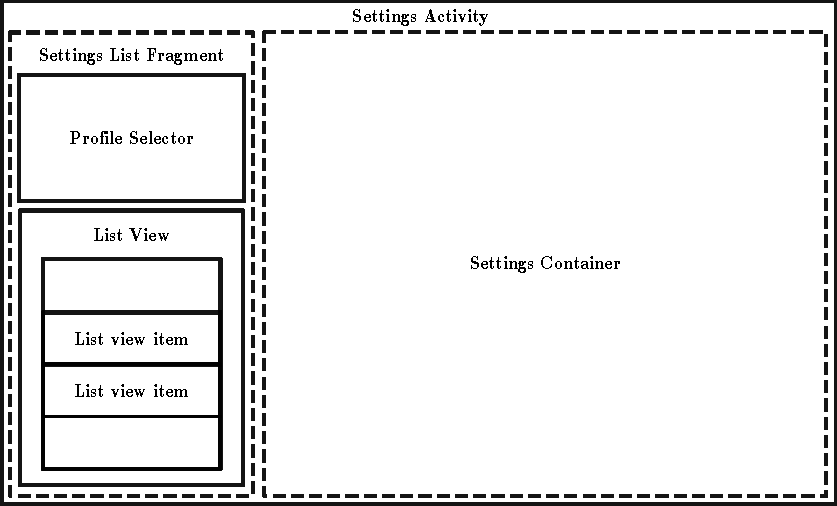
\includegraphics[width=0.8\textwidth, keepaspectratio=true]{SettingsActivity.pdf}
\caption{The architecture showing how the prototype, \cref{fig:settingsprototype}, will be implemented.}
\label{fig:settingsarchitecture}
\end{figure}

Having investigated how to handle settings from other \giraf applications in \cref{sec:sprint3:designsettings}, this section elaborates on how the activity is designed.
The design uses \cref{fig:settingsprototype} as the underlying basis of the decisions.

\paragraph{Settings Activity}
Analogous to opening a new window on a desktop computer, a ``screen'' on an Android device consists of an activity.
\cref{fig:settingsarchitecture} can be compared directly to \Cref{fig:settingsprototype}, expanding on the user interface components that need be included.

To follow Android guidelines, we are using fragments\cite{fragments} to implement the functionality this activity requires. 
They are ideal in this situation, as they are reusable modules which ensure decomposition of the application functionality and user interface.
Managing these with a Fragment Manager, it is also possible to add multiple fragments to a screen without switching activity.

By following these guidelines for developing an activity, it is possible to use the same implementation to show the settings on a smaller screen.
This will be an advantage, should the clients purchase tablets with smaller screens.\\

As illustrated in \cref{fig:settingsarchitecture}, the design consists of one fragment, \textit{Settings List Fragment}, and one container, \textit{Settings Container}.
The settings list fragment contains the profile selector and a list view as described below:
\begin{itemize}
\item \textbf{Profile Selector} is what makes it possible to edit settings for multiple users.
The prototype previously mentioned shows a profile selector resembling a drop-down menu.
To follow the multi-project guidelines, a component developed by the group responsible for \textit{\giraf Components} will be implemented instead.
When the selected profile changes, the settings activity should be reloaded to reflect the settings of the newly selected user.
\item \textbf{ListView} shows the categories of settings which are available to the user.
The fragment attached to each category is presented in the settings container when the category is chosen.
\end{itemize}

\subsection{Launcher Settings}\label{sec:launchersettings}
Following the prototypes from \cref{fig:prototypes}, it is clear that a decision has to be taken regarding which settings to include for \launcher.
According to the client meetings, \cref{sec:sprint2:firstmeeting,sec:sprint2:secondmeeting}, the presented design and its functionality received positive feedback.
To build on this idea, the following settings should be included:

\begin{itemize}
\item \textbf{\launcher settings}\\
Since no critical settings are needed for \launcher, it will contain the settings presented in the prototypes, apart from the ability to change the colour of an application, as mentioned in \cref{sec:sprint2:secondmeeting}.
\item \textbf{Application management}\\
This part of \launcher is more critical as it will be the only way of adding certain applications to a user, whether they be an Android or \giraf application.
Thus, this part has the responsibility of handling all tasks related to application management.
\end{itemize}

This concludes the design of the settings activity and we subsequently describe the implementation.